Prove that for every positive integer $n$, there exists a finite subset of the squares of an infinite chessboard that can be tiled with indistinguishable $1\times 2$ dominoes in exactly $n$ ways.

\textbf{Solution 1} (Valentin)

Take a $(2n-1)\times 4$ rectangle of squares and remove every second square in row $2$ and $3$ as illustrated below:

\[
\underbrace{\begin{aligned}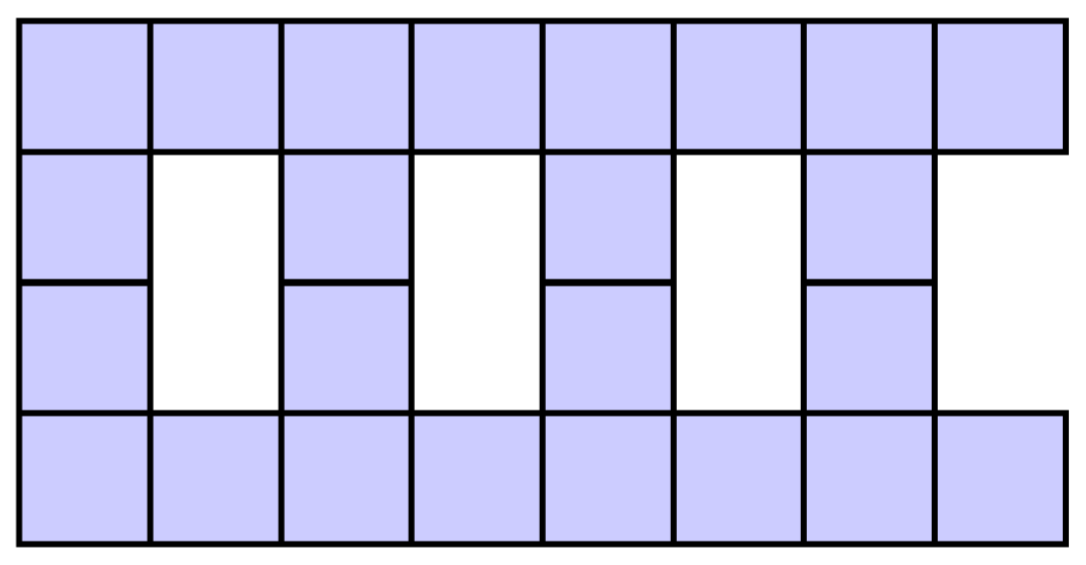
\includegraphics[scale=0.3]{solutions/polyomino_left.png}\end{aligned} \bullet\bullet\bullet\begin{aligned}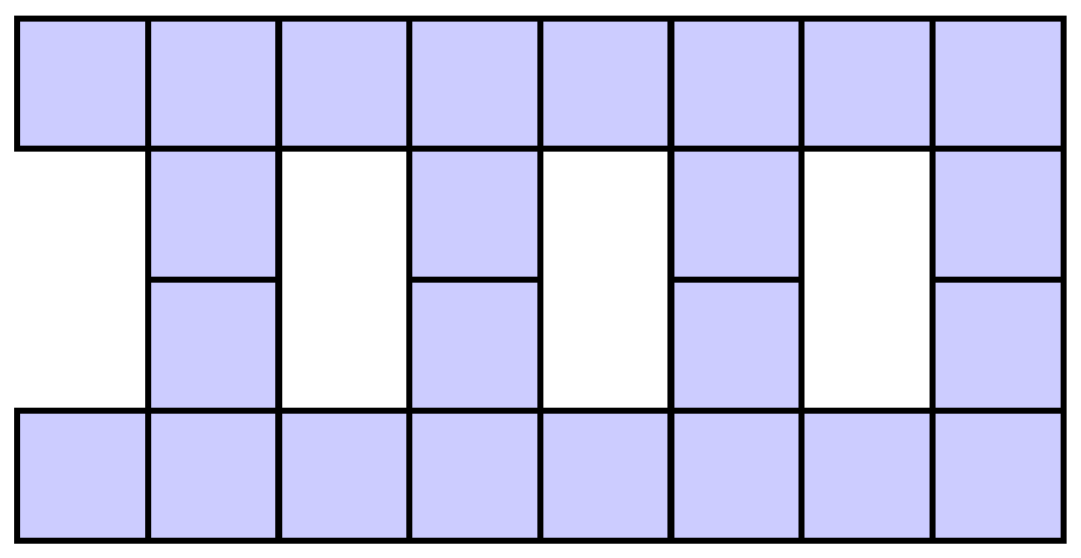
\includegraphics[scale=0.3]{solutions/polyomino_right.png}\end{aligned}}_{\displaystyle2n-1}
\]

Let us now consider an arbitrary tiling of this subset.

\emph{Claim:}
Of all the dominoes overlapping the first row, exactly one is vertical.

\begin{proof}
If all of these dominoes were horizontal, they would cover a total of $2n$ squares in the first row. But since the first row only contains $2n-1$ squares, this is not possible.

If more than one of these dominoes are vertical, choose two of these vertical dominoes $D_1$ and $D_2$ such that all dominoes overlapping the first row between the two are horizontal. The total number of squares covered in the first row by the dominoes between $D_1$ and $D_2$ is even, however the total number of squares in the first row between $D_1$ and $D_2$ is odd, a contradiction.

We conclude that exactly one of the dominoes overlapping the first row is vertical.
\end{proof}

Now every of the $n$ choices for which domino in the first row is vertical leads to a uniquely defined tiling of the whole subset since all the dominoes in row $2$ and $3$ have to be vertical and the bottom row can be uniquely tiled with one vertical domino and $n-1$ horizontal dominoes.

Since every tiling must also exactly have one vertical domino in the first row, we conclude that there are exactly $n$ tilings of this subset.

\newpage

\textbf{Solution 2} (Valentin)

For any $n\geq 2$, consider the two subsets
\[
\left.\begin{aligned}
A_{2n-1}= \begin{aligned}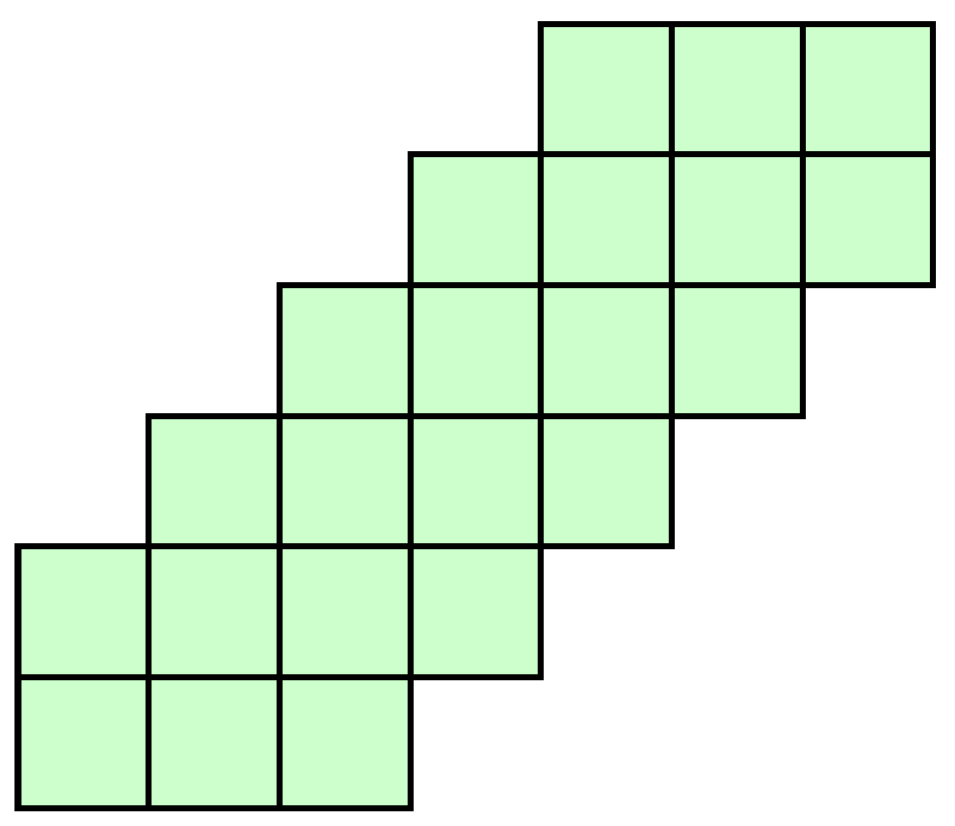
\includegraphics[scale=0.2]{solutions/polyomino-staircase1.png}\end{aligned}
\end{aligned}\right\rbrace n\qquad\text{and}\qquad
\left.\begin{aligned}
A_{2n}=\begin{aligned}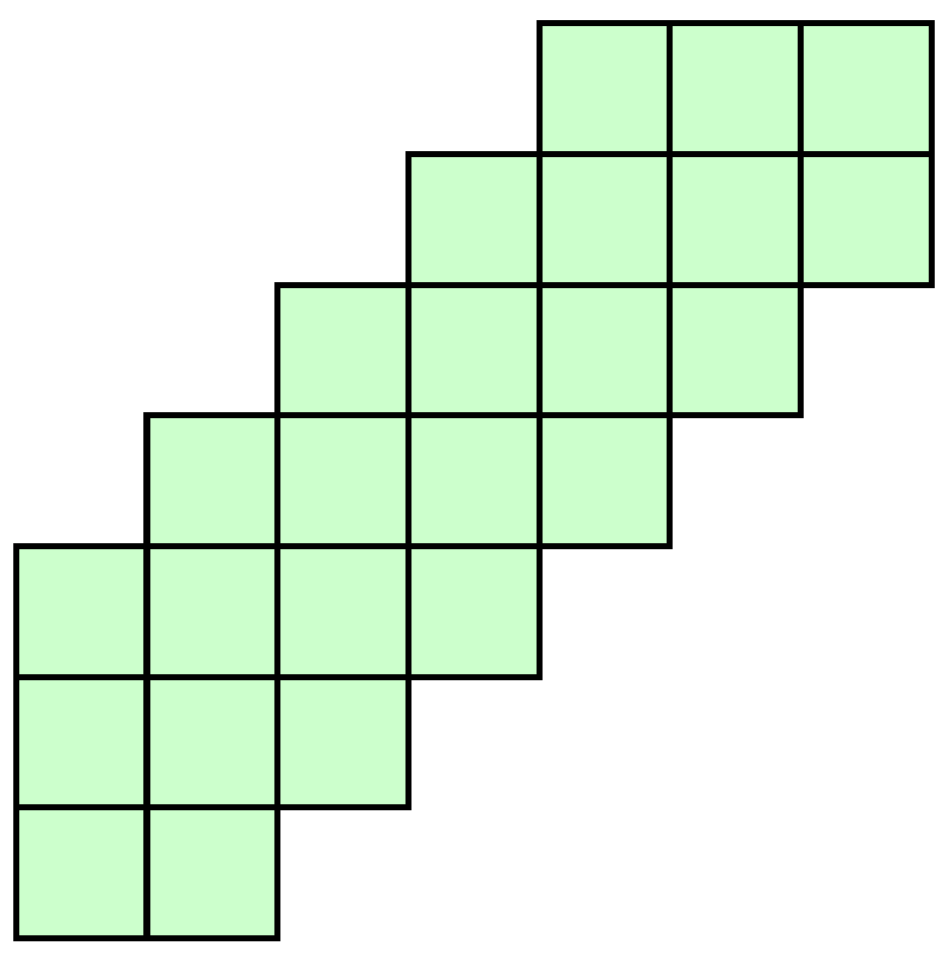
\includegraphics[scale=0.2]{solutions/polyomino-staircase2.png}\end{aligned}
\end{aligned}\right\rbrace n+1
\]

\emph{Claim:}
The subset $A_k$ has exactly $k$ domino tilings for all $k\geq 3$.

\begin{proof}
The claim holds for $k = 3,4$. Now consider $k > 4$.

For $k$ odd, consider $D$, the domino that covers the bottom left square of $A_k$. If $D$ is horizontal, there is only one way of covering the lowest square in each other column, namely by a vertical domino. The remaining squares can only be tiled in one way, namely using only horizontal dominoes. If $D$ is vertical then consider $D'$, the domino that covers the bottom left square of the remaining set. If $D'$ is vertical then similarly to the previous case, there is only one way of tiling the remaining squares. If however $D'$ is horizontal, the remaining set is just $A_{k-2}$. Putting everything together we find that the number of tilings of $A_k$ is the number of tilings of $A_{k-2}$ plus $2$ and we are done by induction.

For even $k$, consider again $D$, the domino that covers the bottom left square of $A_k$. If $D$ is vertical, then similarly to the first case for odd $k$ there is only one way of tiling the remaining squares. If $D$ is horizontal, the remaining set is just $A_{k-1}$ and we already know there are $k-1$ ways of tiling these squares. Putting the two together we find that $A_k$ has $k$ tilings.
\end{proof}

This argument solves the problem for all $n\geq 3$. The cases $n = 1,2$ are trivially true by considering $1\times 2$ and $2\times 2$ rectangles.

\bigskip

\textbf{Marking Scheme} (Additive)

\begin{itemize}
\item 3P: Claiming a concrete construction that works for all but finitely many $n$
\end{itemize}
Points for bounding the number of tilings:
\begin{itemize}
\item 2P: Proving that the construction for $n$ has at most $n$ tilings
\item 2P: Proving that the construction for $n$ has at least $n$ tilings
\end{itemize}

In case the construction distinguishes classes of integers (as in Solution 2), the points are split between them accordingly if the approach leads to a (more or less direct) solution.

\begin{itemize}
\item -1P: Finitely many cases missed or missing base case for induction
\item -1P: If not both directions of a bijective argument (as in Solution 1) are justified
\end{itemize}

No points are awarded for merely reducing the problem to primes or other infinite sets like Fibonacci numbers.